
In a collaboration with members of the IRAC Shallow Cluster Survey
\citep{eisenhardt08a}, the Red-Sequence Cluster Survey (RCS) and RCS-2
\citep{gladders05a,yee07a}, the XMM Cluster Survey \citep{sahlen09a},
the Palomar Distant Cluster Survey \citep{postman96a}, the XMM-Newton
Distant Cluster Project \citep{bohringer05a}, and the ROSAT Deep
Cluster Survey \citep[RDCS;][]{rosati99a}, the SCP developed and
carried out a novel supernova survey approach. We aimed to improve
both the efficiency and usefulness of high-redshift SN observations
with \emph{HST} by specifically targeting high-redshift galaxy
clusters. Clusters provide a significant enhancement in the density of
potential SN hosts in \emph{HST}'s relatively small field of view.
Furthermore, the centers of rich clusters are dominated by relatively
dust-free early-type galaxies. SNe discovered in such galaxies offer
an opportunity to reduce the systematic uncertainty associated with
extinction corrections. Here we summarize the survey, named
the \emph{HST} Cluster Supernova Survey (PI Perlmutter; \emph{HST}
program GO-10496) and discuss aspects most relevant to the SN rate
calculation.

\section{Cluster Targets and Survey Strategy}

We used the Advanced Camera for Surveys (ACS) to search for and
observe SNe in 25 of the most massive galaxy clusters available at the
time of the survey. The survey was carried out during \emph{HST} Cycle
14 with observations spanning from July 2005 to December 2006.
Clusters were selected from X-ray, optical and IR surveys and cover
the redshift range $0.9<z<1.46$. Twenty-four of the clusters have
spectroscopically confirmed redshifts and the remaining cluster has a
photometric redshift estimate.  Cluster positions, redshifts and
discovery methods are listed in Table~\ref{tab:clusters}.

%%%%%%%%%%%%%%%%%%% 
% TABLE: CLUSTERS %
%%%%%%%%%%%%%%%%%%%
\begin{table}[thbp]
\caption{Clusters targeted in survey\label{tab:clusters}}
\begin{center}
\begin{footnotesizetabular}{lccccc}
\hline
\hline
ID & Cluster & Redshift & R.A. (J2000) & Decl. (J2000) & Discovery \\
\hline
A & XMMXCS J2215.9-1738 & 1.45 & $22^{\rm h}\,15^{\rm m}\,59^{\rm s}.0$ & $-17^{\circ}\,37'\,59''$ & X-ray      \\
B & XMMU J2205.8-0159   & 1.12 & $22^{\rm h}\,05^{\rm m}\,50^{\rm s}.6$ & $-01^{\circ}\,59'\,30''$ & X-ray      \\
C & XMMU J1229.4+0151   & 0.98 & $12^{\rm h}\,29^{\rm m}\,29^{\rm s}.2$ & $+01^{\circ}\,51'\,21''$ & X-ray      \\
D & RCS J0221.6-0347    & 1.02 & $02^{\rm h}\,21^{\rm m}\,42^{\rm s}.2$ & $-03^{\circ}\,21'\,52''$ & Optical    \\
E & WARP J1415.1+3612   & 1.03 & $14^{\rm h}\,15^{\rm m}\,11^{\rm s}.1$ & $+36^{\circ}\,12'\,03''$ & X-ray      \\
F & ISCS J1432.4+3332   & 1.11 & $14^{\rm h}\,32^{\rm m}\,28^{\rm s}.1$ & $+33^{\circ}\,33'\,00''$ & IR-Spitzer \\
G & ISCS J1429.3+3437   & 1.26 & $14^{\rm h}\,29^{\rm m}\,17^{\rm s}.7$ & $+34^{\circ}\,37'\,18''$ & IR-Spitzer \\
H & ISCS J1434.4+3426   & 1.24 & $14^{\rm h}\,34^{\rm m}\,28^{\rm s}.6$ & $+34^{\circ}\,26'\,22''$ & IR-Spitzer \\
I & ISCS J1432.6+3436   & 1.34 & $14^{\rm h}\,32^{\rm m}\,38^{\rm s}.8$ & $+34^{\circ}\,36'\,36''$ & IR-Spitzer \\
J & ISCS J1434.7+3519   & 1.37 & $14^{\rm h}\,34^{\rm m}\,46^{\rm s}.0$ & $+35^{\circ}\,19'\,36''$ & IR-Spitzer \\
K & ISCS J1438.1+3414   & 1.41 & $14^{\rm h}\,38^{\rm m}\,08^{\rm s}.2$ & $+34^{\circ}\,14'\,13''$ & IR-Spitzer \\
L & ISCS J1433.8+3325   & 1.37 & $14^{\rm h}\,33^{\rm m}\,51^{\rm s}.1$ & $+33^{\circ}\,25'\,50''$ & IR-Spitzer \\
M & Cl J1604+4304       & 0.92 & $16^{\rm h}\,04^{\rm m}\,23^{\rm s}.8$ & $+43^{\circ}\,04'\,37''$ & Optical    \\
N & RCS J0220.9-0333    & 1.03 & $02^{\rm h}\,20^{\rm m}\,55^{\rm s}.5$ & $-03^{\circ}\,33'\,10''$ & Optical    \\
P & RCS J0337.8-2844    & 1.1$^{\rm a}$ & $03^{\rm h}\,37^{\rm m}\,51^{\rm s}.2$ & $-28^{\circ}\,44'\,58''$ & Optical    \\
Q & RCS J0439.6-2904    & 0.95 & $04^{\rm h}\,39^{\rm m}\,37^{\rm s}.6$ & $-29^{\circ}\,05'\,01''$ & Optical    \\
R & XLSS J0223.0-0436   & 1.22 & $02^{\rm h}\,23^{\rm m}\,03^{\rm s}.4$ & $-04^{\circ}\,36'\,14''$ & X-ray      \\
S & RCS J2156.7-0448    & 1.07 & $21^{\rm h}\,56^{\rm m}\,42^{\rm s}.2$ & $-04^{\circ}\,48'\,04''$ & Optical    \\
T & RCS J1511.0+0903    & 0.97 & $15^{\rm h}\,11^{\rm m}\,03^{\rm s}.5$ & $+09^{\circ}\,03'\,09''$ & Optical    \\
U & RCS J2345.4-3632    & 1.04 & $23^{\rm h}\,45^{\rm m}\,27^{\rm s}.2$ & $-36^{\circ}\,32'\,49''$ & Optical    \\
V & RCS J2319.8+0038    & 0.91 & $23^{\rm h}\,19^{\rm m}\,53^{\rm s}.4$ & $+00^{\circ}\,38'\,13''$ & Optical    \\
W & RX J0848.9+4452     & 1.26 & $08^{\rm h}\,48^{\rm m}\,56^{\rm s}.4$ & $+44^{\circ}\,52'\,00''$ & X-ray      \\
X & RDCS J0910+5422     & 1.11 & $09^{\rm h}\,10^{\rm m}\,45^{\rm s}.1$ & $+54^{\circ}\,22'\,07''$ & X-ray      \\
Y & RDCS J1252.9-2927   & 1.23 & $12^{\rm h}\,52^{\rm m}\,54^{\rm s}.4$ & $-29^{\circ}\,27'\,17''$ & X-ray      \\
Z & XMMU J2235.3-2557   & 1.39 & $22^{\rm h}\,35^{\rm m}\,20^{\rm s}.8$ & $-25^{\circ}\,57'\,39''$ & X-ray      \\


\hline
\end{footnotesizetabular}
\end{center}
{\footnotesize

$^{\rm a}$ photometric redshift

{\bf References.} --- A \citep{stanford06a,hilton07a}; 
B,C \citep{bohringer05a,santos09a}; 
D \citep[also known as RzCS 052;][]{andreon08b,andreon08c}; 
D, N, U (Gilbank et al. in prep); E \citep{perlman02a};
F \citep{elston06a}; G, I, J, L \citep{eisenhardt08a}; 
L (Brodwin et al. in prep; Stanford et al. in prep);
H \citep{brodwin06a}; K \citep{stanford05a}; M \citep{postman01a};
Q \citep{cain08a}; R \citep{andreon05a,bremer06a};
S \citep{hicks08a}; V \citep{gilbank08a}; W \citep{rosati99a};
X \citep{stanford02a}; Y \citep{rosati04a}; 
Z \citep{mullis05a,rosati09a}.\\
{\bf Note.} --- Cluster positions differ slightly from those
originally reported in \citet{dawson09a} due to the use of an updated
algorithm for determining cluster centers. See \S\ref{sec:lum}
for a description of this algorithm.
}
\end{table}

During the survey, each cluster was observed once every 20 to 26 days
during its \emph{HST} visibility window (typically four to seven
months). Figure~\ref{fig:visits} shows the dates of visits to
each cluster. Each visit consisted of four exposures in the F850LP
filter (hereafter $z_{850}$).  Most visits also included a fifth
exposure in the F775W filter (hereafter $i_{775}$). We revisited
clusters D, N, P, Q, R and Z towards the end of the survey when they
became visible again.

%%%%%%%%%%%%%%%%
% PLOT: VISITS %
%%%%%%%%%%%%%%%%

\begin{SCfigure}[0.7][thb]
\centering
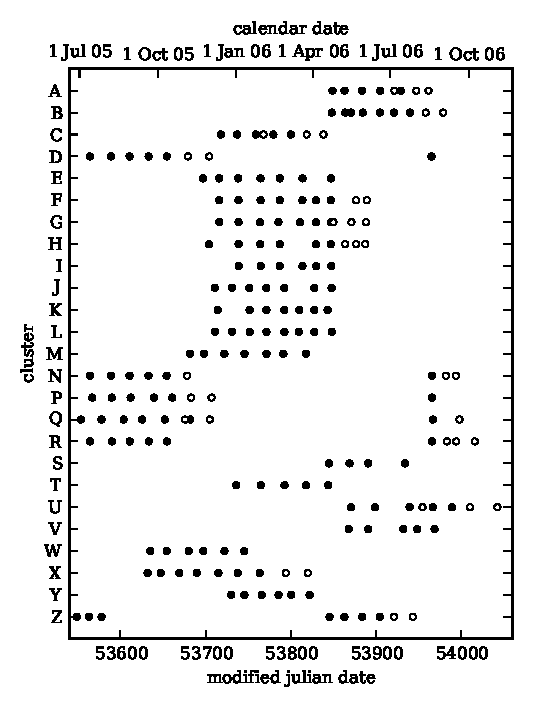
\includegraphics{figures/survey/visits.eps}
\caption[Dates of visits to each cluster]{Dates of visits to each
  cluster. All visits included $z_{850}$ exposures (usually
  four). Most visits also included one $i_{775}$ exposure. Filled
  circles indicate ``search'' visits (used for finding SNe). Open
  circles indicate ``follow-up'' visits (contingent on the existence
  of an active SN candidate). Clusters D, N, P, Q and R were
  re-visited once towards the end of the survey, with additional
  follow-up visits devoted to clusters in which promising SN
  candidates were found (N, Q, R). \label{fig:visits}}
\end{SCfigure}


Immediately following each visit, the four $z_{850}$ exposures were
cosmic ray-rejected and combined using {\sc MultiDrizzle}
\citep{fruchter02a,koekemoer02a} and searched for
supernovae. Following the technique employed in the earliest Supernova
Cosmology Project searches \citep{perlmutter95a,perlmutter97a}, we
used the initial visit as a reference image, flagged candidates with
software and then considered them by eye. Likely supernovae were
followed up spectroscopically using pre-scheduled time on the Keck
and Subaru telescopes and target-of-opportunity observations on VLT.
For nearly all SN candidates, either a live SN spectrum or host galaxy
spectrum was obtained. In many cases, spectroscopy of cluster galaxies
was obtained contemporaneously using slit masks. Candidates deemed
likely to be at higher redshift ($z>1$) were also observed with the
NICMOS camera on {\it HST}, but these data are not used in this work.

For the purpose of a rate calculation it is important to note that a
number of visits were contingent on the existence of an active SN. At
the end of a cluster's visibility window, the last two scheduled
visits were cancelled if there was no live SN previously
discovered. This is because a SN discovered on the rise in either of
the last two visits could not be followed long enough to obtain a
cosmologically useful light curve. In addition, supplementary visits
between pre-scheduled visits were occasionally added to provide more
complete light curve information for SNe (in the case of clusters A,
C, Q, and U). We call all visits contingent on the existence of an
active SN ``follow-up'' visits (designated by open circles in
Fig.~\ref{fig:visits}). Search and follow-up visits are considered
differently when calculating an SN rate.

\section{Data Processing}

Following the conclusion of the survey, all ACS images were
reprocessed \citep[see details in][]{suzuki11a}. This
reprocessing included an updated flat field, gain adjustment, custom
sky subtraction, and updated distortion correction and zeropoints.
The images for each cluster were aligned and output to a single common
reference frame for the cluster using the {\sc MultiDrizzle}
software. That is, the combined images for each epoch are all on the
same image and physical reference frame for a given cluster. This
makes it possible to stack and subtract images without resampling the
data. The four individual exposures (not cosmic ray-rejected) are also
transformed onto this output reference frame. The output pixel scale
is equal to the physical pixel scale: $0''.05$.

A single sky noise for each image is calculated, for use in the rate
calculation. To do this accurately, we first cut pixels with effective
exposure time less than 50\% of the total exposure time. We calculate
a rough sky noise level, then cut pixels belonging to objects. The
requirement to be an object is 1 pixel above $4\sigma$ and 5
contiguous pixels above $2.5\sigma$. This is done iteratively until
$\sigma$ has converged to within 25\%.

\section{Survey Publications}

The supernova-related results from the survey are reported in the
following publications: Paper I \citep{dawson09a} describes the survey
strategy and discoveries. Paper II \citep{barbary11a} reports on the
SN~Ia rate in clusters. Paper III \citep{meyers11a} addresses the
properties of the galaxies that host SNe~Ia. Paper
IV \citep{ripoche11a} introduces a new technique to calibrate the
zeropoint of the NICMOS camera at low counts rates, critical for
placing NICMOS-observed SNe~Ia on the Hubble diagram. Paper
V \citep{suzuki11a} reports the SNe~Ia light curves and cosmology from
the program. Paper VI (Barbary et al., in preparation) reports on the
volumetric field SN~Ia rate. \citet{melbourne07a}, one of several
unnumbered papers in the series, present a Keck adaptive optics
observation of a $z=1.31$ SN~Ia in $H$-band. \citet{barbary09a} report
the discovery of the extraordinary luminous supernova,
SN~SCP06F6. \citet{morokuma10a} presents the spectroscopic follow-up
observations for SN candidates. Finally, Hsiao et al. (in preparation)
develop techniques to remove problematic artifacts remaining after the
standard STScI pipeline. A separate series of papers, ten to date,
reports on cluster studies from the survey:
\citet{hilton07a,eisenhardt08a,jee09a,hilton09a,huang09a,rosati09a,
santos09a,strazzullo10a,brodwin10a}; Jee et al. (in preparation).
